\documentclass{minimal}
\usepackage{graphicx,color}
\usepackage[utf8]{inputenc}
\usepackage[papersize={419.00bp,332.00bp},text={419.00bp,332.00bp}]{geometry}
\begin{document}
\centering
% Title: gl2ps_renderer figure
% Creator: GL2PS 1.4.2, (C) 1999-2020 C. Geuzaine
% For: Octave
% CreationDate: Mon Dec 12 16:51:23 2022
\setlength{\unitlength}{1pt}
\begin{picture}(0,0)
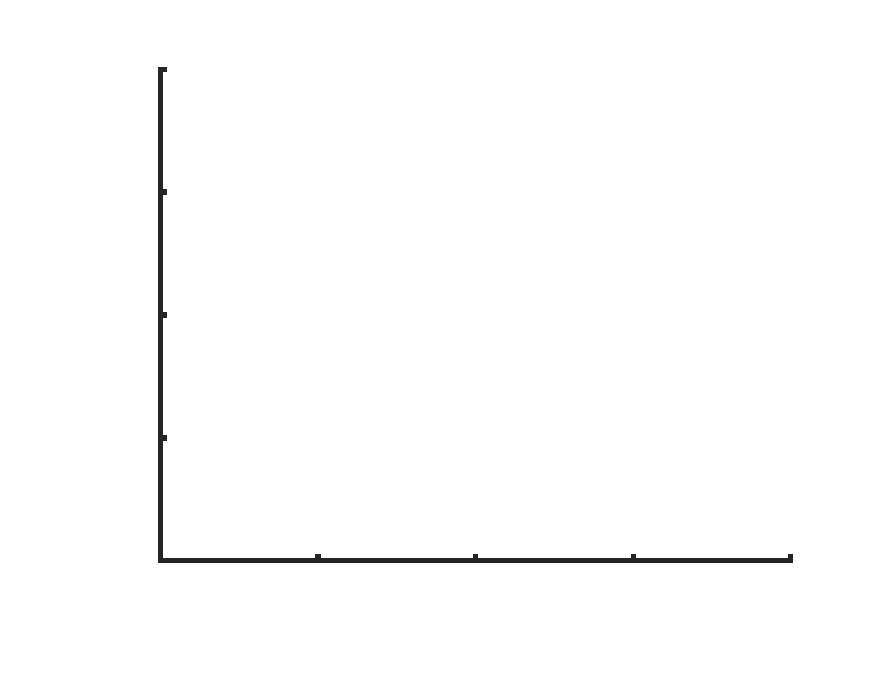
\includegraphics[scale=1]{DoubleKapitzaPoincareMapped-inc}
\end{picture}%
\begin{picture}(419,332)(0,0)
\fontsize{22}{0}\selectfont\put(76.986,46.4376){\makebox(0,0)[t]{\textcolor[rgb]{0.15,0.15,0.15}{{-1}}}}
\fontsize{22}{0}\selectfont\put(152.64,46.4376){\makebox(0,0)[t]{\textcolor[rgb]{0.15,0.15,0.15}{{-0.5}}}}
\fontsize{22}{0}\selectfont\put(228.293,46.4376){\makebox(0,0)[t]{\textcolor[rgb]{0.15,0.15,0.15}{{0}}}}
\fontsize{22}{0}\selectfont\put(303.947,46.4376){\makebox(0,0)[t]{\textcolor[rgb]{0.15,0.15,0.15}{{0.5}}}}
\fontsize{22}{0}\selectfont\put(379.601,46.4376){\makebox(0,0)[t]{\textcolor[rgb]{0.15,0.15,0.15}{{1}}}}
\fontsize{22}{0}\selectfont\put(66,62.9417){\makebox(0,0)[r]{\textcolor[rgb]{0.15,0.15,0.15}{{-1}}}}
\fontsize{22}{0}\selectfont\put(66,121.956){\makebox(0,0)[r]{\textcolor[rgb]{0.15,0.15,0.15}{{-0.5}}}}
\fontsize{22}{0}\selectfont\put(66,180.971){\makebox(0,0)[r]{\textcolor[rgb]{0.15,0.15,0.15}{{0}}}}
\fontsize{22}{0}\selectfont\put(66,239.985){\makebox(0,0)[r]{\textcolor[rgb]{0.15,0.15,0.15}{{0.5}}}}
\fontsize{22}{0}\selectfont\put(66,299){\makebox(0,0)[r]{\textcolor[rgb]{0.15,0.15,0.15}{{1}}}}
\fontsize{24}{0}\selectfont\put(228.293,24.4376){\makebox(0,0)[t]{\textcolor[rgb]{0.15,0.15,0.15}{{$\theta_2/(2 \pi)$}}}}
\fontsize{24}{0}\selectfont\put(24,180.971){\rotatebox{90}{\makebox(0,0)[b]{\textcolor[rgb]{0.15,0.15,0.15}{{$\omega_2$}}}}}
\fontsize{24}{0}\selectfont\put(228.293,309){\makebox(0,0)[b]{\textcolor[rgb]{0,0,0}{{Poincaré Section at $\theta_1 = 0$}}}}
\end{picture}
\end{document}
